\documentclass[captions=tableheading,
  bibliography=totoc,
  titlepage=firstiscover
  ]{scrartcl}
\usepackage{scrhack}

\usepackage[a4paper,top=2.5cm,left=2.5cm,right=2cm,bottom=3cm,bindingoffset=5mm]{geometry}

\usepackage[aux]{rerunfilecheck}

\usepackage{polyglossia}
\setmainlanguage{german}

\usepackage{amsmath}
\usepackage{amssymb}
\usepackage{mathtools}

\usepackage{fontspec}

\usepackage{biblatex}
\addbibresource{lit.bib}  %nach polyglossia

\usepackage[
  math-style=ISO,
  bold-style=ISO,
  sans-style=italic,
  nabla=upright,
  partial=upright,
]{unicode-math}

\usepackage[
  locale=DE,
  separate-uncertainty=true,
  per-mode=symbol-or-fraction,
]{siunitx}

\usepackage[section, below]{placeins}
\usepackage[
  labelfont=bf,        % Tabelle x: Abbildung y: ist jetzt fett
  font=small,          % Schrift etwas kleiner als Dokument
  width=0.9\textwidth, % maximale Breite einer Caption schmaler
  format=plain,
  indention=1em, % Abbildung sticht links etwas hervor
]{caption}
\usepackage{graphicx}
\usepackage{grffile}
\usepackage{subcaption}

\usepackage{booktabs}
\usepackage{float}
\floatplacement{figure}{htbp}
\floatplacement{table}{htbp}


\usepackage[unicode]{hyperref}
\usepackage{bookmark}
\usepackage{microtype}


\title{V303 - Der Lock-In-Verstärker}
\author{Julian Jung \\ julian.jung@tu-dortmund.de
  \and Pascal Gutjahr \\ pascal.gutjahr@tu-dortmund.de}
  \date{Durchführung: 18.11.2016
  \hspace{3em}
  Abgabe: 25.11.2016 \\
  1. Korrektur: 09.12.2016}
  \begin{document}
\maketitle
\newpage
\tableofcontents
\newpage
\section{Zielsetzung}
Der Versuch dient der Einführung in die Funktion eines Lock-In-Verstärkers.
Hierfür werden die einzelnen Bauteile des Verstärkers einzeln angesteuert und
auf ihre Funktion überprüft.
\section{Theorie}
Mit dem Franck-Hertz-Versuch lässt sich die die Quantennatur der Elektronenhülle
eines Atoms bestimmen. Es bestätigte zudem die
Bohr'schen Postulate. Somit lassen sich Widersprüche auflösen, die zwischen
der Maxwellschen Elektrodynamik und der Atomspektroskopie bestehen.

Bei dem Franck-Hertz-Versuch handelt es sich um ein Elektronenstoßexperiment.
Hierbei werden Atome mit Elektronen mit geeigneter Energie beschossen werden.
Als Informationsquelle dient der Energieverlust der Elektronen. Durch die Wechselwirkung
von monoenergetischen Elektronen mit Hg-Dampf kommt es sowohl zu elastischen, als
auch zu unelastischen Stößen. Die vom
Quecksilber aufgenommene Energie wird hierbei mit der Energiedifferenz der
Elektronen vor und nach dem Stoß berechnet. Diese Energie wird beim unelastischen
Stoß dazu verwendet, um das Hg-Atom aus seinem Grundzustand $E_0$ in den ersten angeregten
Zustand $E_1$ zu heben. Es gilt:
\begin{equation}
  \frac{\su{m_0\cdot v_{vor}^2}}{2}-\frac{\su{m_0\cdot v_{nach}^2}}{2} = E_1-E_0.
\end{equation}

In einem evakuierten Gefäß verdampft ein Tropfen Quecksilber, bis sich ein
Sättigungsdruck $p_{sat}$ einstellt, der abhängig von der Temperatur $T$ ist. Die 
Temperatur ist somit maßgbend für die Dampfdichte.
In einem Glaskolben befindet sich ein Draht, welcher bis zur Rotglut erhitzt
wird. Durch den Glühelektrischen Effekt treten Elektronen in großer Zahl aus und
bilden eine Art Wolke, die den Draht umgibt. An der Elektrode gegenüber dem Glühdraht wird
eine positive Gleichspannung $U_\su{B}$ angelegt. Die kinetische Energie der
Elektronen nach dem durchlaufen dieser Strecke beträgt
\begin{equation}
  \frac{\su{m_0\cdot v_{vor}^2}}{2}.
  \label{Ekin}
\end{equation}
Hinter dieser Elektrode befindet sich eine weitere Elektrode an der ein
Auffängerstrom $I_\su{A}$ und eine geringere Gegenspannung $U_\su{A}$ angelegt
ist. Es gelangen jedoch nur Elekronen zu dieser Auffängerelektrode, deren
Geschwindigkeitskomponente $v_\su{z}$ die Ungleichung
\begin{equation}
  \frac{\su{m_0}}{2}v_\su{z}^2 \geq e_0U_\su{A}
\end{equation}
erfüllt. Erfüllt ein Elektron diese Ungleichung nicht, kehrt es zur
Beschleunigerelektrode zurück. Die Hg-Atome die sich nun im Beschleunigungsraum
aufhalten stoßen mit Elektronen zusammen. Hierbei werden 2 Fälle unterschieden.
Elastische Stöße treten hierbei nur auf, wenn die Energie der Elektronen
nicht allzu groß ist. Die
Energie, die das Elektron an das Hg-Atom abgibt ist hierbei vernachlässigbar
gering. Diese beträgt im zentralen Stoß
\begin{equation}
  \Delta E = \frac{\su{4m_0M}}{\su{(m_0+M)^2}}E\approx 1.1\,\cdot10^{-5}E.
\end{equation}
Dies liegt an dem Masseverhältnis $\frac{m_0}{M} von Elektron und Quecksilber,
welches etwa $1/1836\,\cdot201$\cite{601} beträgt. 

Erreicht die Elektronenenergie einen Wert der größer oder gleich der
Energiedifferenz zwischen dem Grundzustand und dem ersten angeregtem Zustand,
kann das Elektron das Quecksilberatom anregen. Hierbei überträgt das Elektron
genau den Energiebetrag $E_1-E_0$ auf die Elektronenhülle des Hg-Atoms.
Die Zeit die das Hg-Atom braucht um in den Grundzustand zurückzukehren liegt
in der Größenordnung von $10^{-8}\sek$
Die Energie des emittierten Lichtquants liegt bei
\begin{equation}
  \su{h}\nu =E_1-E_0.
\end{equation}
Um festzustellen, wann das Hg-Atom angeregt wird, wird der
Auffängerstrom $I_\su{A}$ in Abhängigkeit der Berschleunigerspannung $U_\su{B}$
beobachtet. Der Elektronenstrom wächst an, wenn die Beschleunigerspannung die
Auffängerspannung übersteigt.

Wenn die Elektronenenergie den Wert $E_1-E_0$ erreicht oder überschreitet, treten
unelastische Stöße auf, bei denen die Elektronen praktisch ihre gesamte Energie
abgeben und somit nicht mehr gegen das Bremsfeld anlaufen können.
Somit muss der Auffängerstrom stark absinken.
Wenn die Beschleunigerspannung $U_\su{B}$ weiter gesteigert wird, können die
Elektronen wieder Energie aufnehmen. Dies liegt an der Stoßzone, welche nun nur
knapp vor der Beschleunigerelektrode liegt.
Der Auffängerstrom steigt nun wieder an, bis die Elektronen die Energie $E_1-E_0$
erreicht haben und einen weiteren uneleastischen Stoß anregen können.
Dieser Vorgang lässt sich bei weiterer Steigerung von $U_\su{B}$ noch einige
Male wiederholen. Der Verlauf des Auffängerstroms in Abhängigkeit zur
Beschleunigungsspannung ist in der unten stehenden Abbildung \ref{fig:kurve} zu
sehen.
\begin{figure}
  \centering
  \includegraphics[width=0.8\textwidth]{bilder/kurve.pdf}
  \caption{Idealisierte Franck-Hertz-Kurve zwischen $I_A$ und $U_B$
  \cite{601}.}
  \label{fig:kurve}
\end{figure}
Der Abstand zweier Maxima $U_1$ ist gleich dem ersten Anregungspotential
\begin{equation*}
  U_1:=\frac{1}{e_0}(E_1-E_0)
\end{equation*}
des Quecksilber-Atoms.
Der tatsächliche Verlauf der Franck-Hertz-Kurve aus Abbildung \ref{fig:kurve}
wird von verschiedenen Nebeneffekten beeinflusst.

Da die Austrittsarbeit für Elektronen verschieden ist, unterscheidet sich das
tatsächliche Beschleunigungspotential von U_\su{B}.
Damit die Emissionsrate auch bei kleinen Temperaturen hoch ist, muss die
Austrittsarbeit des Drahts $\Phi_\su{G}$ viel kleiner sein als die
Austrittsarbeit der Beschleunigungselektrode $\Phi_\su{B}$.
\newpage
Abbildung \ref{fig:pot} zeigt die Potentialverhältnisse zwischen beiden Elektroden
\begin{figure}
  \centering
  \includegraphics[width=0.8\textwidth]{bilder/potential.pdf}
  \caption{Potentialverhältnisse zwischen Glühkathode und Beschleunigungselektrode
  \cite{601}.}
  \label{fig:pot}
\end{figure}
Nach dieser Abbildung berechnet sich das tatsächliche Beschleunigungspotential
mittels
\begin{equation}
  U_\su{B,eff}=U_\su{B}-\frac{1}{e_0}(\Phi_\su{B}-\Phi_\su{G}).
\end{equation}
Das Kontaktpotential
\begin{equation}
  K:= \frac{1}{e_0}(\Phi_\su{B}-\Phi_\su{G})
\end{equation}
gibt die Verschiebung der Franck-Hertz-Kurve an.

Desweiteren wurde bisher angenommen, dass die Elektronen nach durchlaufen des
Beschleunigungsraums alle die eine einheitliche Energie besitzen. Da die
Leitungselektronen bereits ein Potential besitzen, treten sie bei der
Glühemission mit unterschiedlichen Anfangsgeschwindigkeiten aus.
Die Leitungselektronen besitzen nach dem Durchlaufen des Beschleunigerpotentials $U_\su{B,eff}$
eine bei $U_\su{B} beginnende Energieverteilung, welche sich zu höheren Energien erstrecken kann.
Das führt dazu, dass sich der Ort der elastischen
Stöße über einen unendlichen Einsatzbereich erstrecken. Die Franck-Hertz-Kurve nähert sich einem
Stromminimum an und fällt nicht, wie in Abbildung \ref{fig:kurve} auf einen Ausgangswert von $0$
zurück. 
Die elastischen Stöße führen zu einer Abflachung und Verbreiterung
der Kurve, sofern sie zwischen den beiden Elektroden stattfinden.

Ein weiterer Nebeneffekt, der die Kurve beeinflusst, ist der Dampfdruck.

Damit die nötigen Zusammenstöße zwischen Elektronen und Hg-Atomen in hohem Maße
auftreten, muss die mittlere Weglänge $\bar w$ sehr klein gegen den Abstand $a$
zwischen Kathode und Beschleunigungselektrode sein. Die Weglänge kann über
den Sättigungsdruck eingestellt werden. Aus der kinetischen Gastheorie folgt der
Zusammenhang
\begin{equation}
  \bar w = \frac{0.0029}{\su{p_{sät}}}
  \label{eqn:wbar}.
\end{equation}

\begin{figure}
  \centering
  \includegraphics[height=0.8\textwidth]{bilder/dampf.pdf}
  \caption{Ideale Quecksilber-Dampfdruckkurve\cite{601}.}
  \label{fig:dampf}
\end{figure}
Die in Abbildung \ref{fig:dampf} gezeigte Dampfdruckkurve von Quecksilber
lässt sich mit
\begin{equation}
  \su{p_{sät}(T)=5.5\,\cdot10^{-7}\,\exp^{-6876/T}}
  \label{eqn:psat}
\end{equation}
berechnet.Die Temperatur bei welcher der Franck-Hertz-Effekt auftritt lässt sich
so berechnen.. Damit eine ausreichende Stoßwahrscheinlichkeit
gegeben ist, muss $\bar w$ um den Faktor 1000 bis 4000 kleiner sein als $a$
sein.
Somit gibt es einen Dampfdruckbereich bei dem eine optimale Arbeit der Apparatur gewährleistet ist.
Wird dieser unterschritten, steigt die Wahrscheinlichkeit, dass die Elektronen
keine Wechselwirkung erfahren.
Ist die Elektronenenergie bei ausreichend hoher Spannung größer als $E_1-E_0$,
können die Hg-Atome in höhere Niveaus angeregt werden.
ist der Sättigungsdruck zu groß, treten zu viele elastische Stöße auf und die Zahl
der Elektronen nimmt stark ab.

Das Hg-Atom besteht aus 80 Elektronen, die sich auf die abgeschlossenen Schalen
des Xe-Atoms mit 54 Elektronen, eine 4f-Schale mit 14 Elektronen und eine
5d-Schale mit 10 Elektronen verteilen. Diese Schalen sind ebenfalls abgeschlossen. Von Bedeutung
sind hierbei jedoch nur die 2s-Elektronen die sich in der Schale mit der
Hauptquantenzahl $n=6$ aufhalten. Die Spins dieser müssen wegen des
Pauli-Verbots im Grundzustand antiparallel stehen, da sonst alle 4
Quantenzahlen übereinstimmen würden.
Die beiden äußersten Elektronen des Hg-Atoms besitzen somit die
Quantenzahlen
\begin{align*}
  n_1 &= n_2 = 6, \\
  l_1 &= l_2 = 0, \\
  s_1 &= \frac{1}{2}, \\
  s_2 &= - \frac{1}{2}.
\end{align*}
Der Grundzustand besitzt demnach keine Feinstruktur, da die Gesamtspinquantenzahl
$S$ verschwindet. Unter Beibehaltung von $S=0$ sind Übergänge in angeregte
zustände nur möglich, wenn die Hauptquantenzahl $n=6$ auf $n=7$ erhöht wird
und $l_1$ wegen der Auswahlregel von 0 auf 1 übergeht. Wird die Anforderung
$S=0$ vernachlässigt, lässt sich ein Niveau erzeugen, bei dem beide Spins
parallel stehen. Hierfür muss zudem der Bahndrehimpuls eines der beiden
Elektronen um 1 ändern, womit $L=1$ gilt. Das so entstandene Niveau besitzt
eine Feinstruktur aus 3 Niveaus, da 3 verschiedene Kombinationen von
$\su{\vec{L}}$ und $\su{\vec{S}}$ vorhanden sind, die zu einem Gesamtrehimpuls
$\su{\vec{J}}$ führen. Durch die Parallelstellung der Spins vermindert sich
die potentielle Energie der Elektronenhülle, da die Elektronen sich gegenseitig
"ausweichen". Das hat zur Folge, dass die Niveaus mit $n=7$ und $S=0$ unterhalb
dem Niveau mit $n=7$ und $S=1$ liegen. Die nachfolgenden Abbildung \ref{fig:termschema}
veranschaulicht die auftretenden Energierelationen.
\begin{figure}
  \centering
  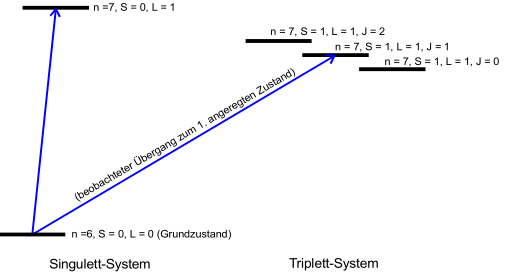
\includegraphics[width=0.7\textwidth]{bilder/term.jpg}
  \caption{Termschema des Hg-Atoms \cite{601}.}
  \label{fig:termschema}
\end{figure}
Der eingezeichnete Übergang vom Grundzustand in den 1. angeregten Zustand und
wieder zurück ist bei Atomen mit kleiner Ordnungszahl $z$, wie etwa Helium,
praktisch unmöglich. Bei Atomen mit großer Ordnungszahl, zum Beispiel Hg, ist
dieser Vorgang nur mit geringer Wahrscheinlichkeit zu beobachten, da er mit dem
Umklappen  eines Elektronenspins, also $\Delta s=1$, verbunden ist. Beim
Franck-Hertz-Experiment ist dies jedoch möglich, da die Anregung durch
Elektronenstoß erfolgt. Das stoßende Elektron wird hier gegen eines der beiden
6s Elektronen ausgetauscht, deren Spinrichtung entgegengesetzt ist.

\section{Aufbau und Durchführung}
\subsection{Vorbereitung}
Bevor der eigentliche Versuch beginnt, werden für drei periodische Funktionen
die jeweiligen Fourier-Koeffizienten berechnet.
\subsubsection{Rechteckspannung}
Um die Koeffizienten der Rechteck-Schwingung zu berechnen, wird diese zunächst
als ungerade Funktion definiert, sodass $f(t)=-f(-t)$ gilt. Daraus wird direkt
gefolgert, dass der Koeffizient $a_\su{n}=0$ ist.
Die Rechteckschwingung wird über die Funktion
% \begin{itemize}
  % \item Rechteckspannung
  \begin{align}
  f(t)&=
  \begin{cases}
    1 & \, 0<t<\frac{\pi}{2} \\
    -1& \, \frac{\pi}{2}<t<\pi \\
  \end{cases}
\end{align}
% \end{itemize}
definiert. Nach Formel \eqref{eq:analyse} berechnet sich der Koeffizient $b_\su{n}$
wie folgt:
\begin{align*}
  b_\su{n} &= \frac{2}{\pi}\int^\pi_0{f(t)\sin{\left(\frac{2\pi n t}{\pi}\right)} dt} \\
  &= \frac{2}{\pi}\left(\int_0^{\frac{\pi}{2}}{\sin{(2nt)} dt} -
  \int_{\frac{\pi}{2}}^\pi{\sin{(2nt)} dt}\right) \\
  &= \frac{2}{\pi}\left(\left[-\cos{(2nt)}\frac{1}{2n}\right]_0^{\frac{\pi}{2}} +
  \left[\cos{(2nt)}\frac{1}{2n}\right]_{\frac{\pi}{2}}^\pi\right) \\
  &= \frac{2}{\pi}\left(\frac{-\cos{(n\pi)}+\cos{(0)}+\cos{(2n\pi)}-\cos{(n\pi)}}{2n}\right) \\
  &= \frac{2}{\pi}\left(\frac{-(-1)^n+1+1-(-1)^n}{2n}\right) \\
  &= \frac{2}{\pi}\left(\frac{2}{n}\right) \qquad \text{|für ungerade n}\\
  &= \frac{4}{\pi n}.
\end{align*}
Da $\cos{(2\pi)}=1$ ist, ist der Cosinus auch für jedes ganzzahlige Vielfache von
$2\pi$ gleich 1. Für gerade $n$ folgt $b_\su{k}=0$.
Zudem muss die Startbedingung $a_0$ berechnet werden. Dies geschieht mit der
Formel
\begin{equation*}
  a_0 = \frac{1}{\pi}\int_{-\pi}^\pi{f(t) dt}.
\end{equation*}
Somit ist
\begin{align*}
  a_0 &= \frac{1}{\pi}\int_{-\pi}^\pi{f(t) dt} \\
  &= \frac{2}{\pi}\int_0^{\pi}{f(t) dt} \\
  &= \frac{2}{\pi}\biggl(\int_0^{\frac{\pi}{2}}{1 dt} -
  \int^\pi_{\frac{\pi}{2}}{1 dt}\biggr) \\
  &= \frac{2}{\pi}\left(\biggl[t\biggr]_0^{\frac{\pi}{2}} -
  \biggl[t\biggr]_{\frac{\pi}{2}}^\pi\right) \\
  &= 0
\end{align*}
Mit den berechneten Koeffizienten lautet die Fourier-Reihe für die Rechteckspannung
\begin{equation}
  f(t) = 0 + \sum_{n=1}^\infty{\frac{4}{n\pi}\sin{\left(\frac{2\pi n}{\su{T}}t\right)}}
\end{equation}
\newpage
\subsubsection{Sägezahnspannung}
Die Sägezahnspannung wird als
\begin{equation}
  f(t) = t
\end{equation}
für $-\pi < t < \pi$ als ungerade Funktion definiert. Somit ist $a_\su{n}=0$.
$b_\su{n}$ wird mit Formel \eqref{eq:analyse} bestimmt. Dabei wird genau so vorgegangen, wie bei
der Rechteckspannung. Daraus folgt dann:
\begin{equation}
  b_\su{n} = -\frac{2}{n}(-1)^n
\end{equation}
Für gerade $n$ gilt $b_\su{n} = -\sfrac{2}{n}$ und für ungerade $n$ gilt $b_\su{n} = \sfrac{2}{n}$.
Der Koeffizient $a_0$ beträgt ebenfalls 0, wodurch sich die Funktion mit der Reihe
\begin{equation}
  f(t)= \sum_{k=1}^\infty -\frac{2}{n}(-1)^n \sin{(nt)}
\end{equation}
darstellen lässt.
\subsubsection{Dreieckspannung}
Die Dreieckspannung wird definiert als
\begin{equation}
  f(t)= \pi - |t|
\end{equation}
für $-\pi ≤ t < \pi$. Diese Funktion ist gerade, wodurch diesmal $b_\su{n} = 0$ gilt.
Auch hierbei wird Formel \eqref{eq:analyse} verwendent. Für den Vorfaktor ergibt sich
\begin{equation}
  a_\su{n} = \frac{2(1-(-1)^n)}{\pi n^2}.
\end{equation}
$a_\su{n} = 0$ gilt für gerade $n$, für ungerade $n$ gilt $a_\su{n} = -\sfrac{4}{\pi n^2}$.
Der Startfaktor lautet $a_0 = \pi$. Somit ergibt sich für die Reihe
\begin{equation}
  f(t) = \pi + \sum_{k=1}^\infty \frac{2(1-(-1)^n)}{\pi n^2} \cos{(nt)}.
\end{equation}
\par
\noindent Für die Rechteckspannung und die Sägezahnspannung ergeben sich damit die Zusammenhänge
von $\sfrac{1}{n}$, für die Dreieckspannung ergibt sich $\sfrac{1}{n^2}$.
\subsection{Fourier-Synthese}
Für die Fourier-Synthese werden zunächst zwei Ausgänge des Oberwellengenerators
an das Oszilloskop angeschlossen. Damit alle Ausgänge in Phase geschalten werden
können, wird das Oszilloskop zunächst in den X-Y-Betrieb geschaltet. Um eine
optimale Genauigkeit zu erhalten, werden die einzelnen Amplituden der Oberwellen
auf maximal eingestellt. Nun werden die Phasen so lange variiert, bis sich
Lissajous-Figuren, wie beispielsweise in Abbildung \ref{lissa}, bilden.
\begin{figure}[H]
  \centering
  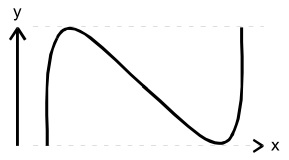
\includegraphics{bilder/lissajous.jpg}
  \caption{Beispiel für eine Lissajous-Figur}
  \label{lissa}
\end{figure}
% Wie es sich in der Vorbereitung
% herausgestellt hat, fallen die Koeffizienten der Funktionen der
% Sägezahn- und Recht-
% eckspannung mit dem Proportionalitätsfaktor X ab.
Die Ausgänge des Oszilloskops werden nun nacheinander an ein Voltmeter
angeschlossen. Die Amplituden der Oberwellen werden entsprechend eingestellt.
Das Oszilloskop wird in den normalen Betrieb zurückgeschaltet und der Generator
an das Oszilloskop angeschlossen. Die einzelnen Oberwellen werden aufaddiert und
gegebenenfalls in der Phase verschoben, bis möglichst genau eine Sägezahnspannung
approximiert wird.
Für die Rechteckspannung wird ähnlich vorgegangen, nur dass jetzt nur die
ungeraden Oberwellen benutzt werden.

Abschließend wird die Durchführung für die Dreieckspannung wiederholt. Hier müssen
zunächst die Amplituden mit dem Proportionalitätsfaktor X eingestellt werden.
Auch hier werden, wie bei der Rechteckspannung, nur die ungeraden Oberwellen
genutzt. Die Phase wird wieder so verschoben, dass die Dreieckspannung möglichst
genau approximiert wird.
\subsection{Fourier-Analyse}
Für die Fourier-Analyse von periodischen Schwingungen wird eine Schaltung wie in
Abbildung \ref{fig:ana} verwendet.
\begin{figure}[h]
  \centering
  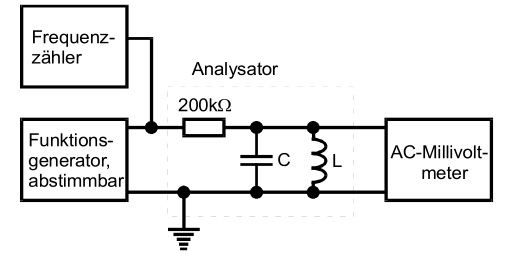
\includegraphics[width=0.8\textwidth]{bilder/analyse.jpg}
  \caption{Schaltung zur Fourier-Analyse\,\cite{351}}
  \label{fig:ana}
\end{figure}
Als Signalquelle dient hier ein durchstimmbarer Funktionsgenerator. Die
Transformation wird direkt vom Oszilloskop durchgeführt.

Damit genügend Peaks des Linienspektrums sichtbar werden, müssen ausreichend
Perioden angezeigt werden. Die angezeigten Peaks werden nun mit einer
Sinusspannung kalibriert und die Frequenz und die Amplitude werden notiert.
Nebenmaxima die sich bilden können, werden nicht beachtet. Die Messung wird für
alle genannten Funktionen durchgeführt.

\section{Auswertung}
Im ersten Aufgabenteil wird eine Referenzspannung von $U_\text{ref}=6.56 \;\si{\volt}$
und eine Signalspannung von $U_\text{sig}=13.5 \;\si{\volt}$ angelegt.
Die Frequenz wird hierbei manuell reguliert und die Spannungsamplituden
$U_\text{SS}$ werden peak-to-peak gemessen.


\begin{table}[!h]
  \centering
  % \begin{subtable}{0.3\textwidth}
  %   \begin{tabular}{S[table-format=4.0]S}
  %     \toprule
  %     {$\varphi$} &
  %     {$U_\text{SS} \,/\, \si{\volt}$} \\
  %     \midrule
  %     15\si{\degree} & 0.82  \\
  %     45\si{\degree} & 0.81 \\
  %     105\si{\degree} & 0.46  \\
  %     165\si{\degree} & 0.88 \\
  %     225\si{\degree} & 0.82  \\
  %     330\si{\degree}  & 0.83  \\
  %     \bottomrule
  %   \end{tabular}
  %   \caption{ohne Tiefpass}
  %   \label{tab:a}
  % \end{subtable}
  % \quad
  % \begin{subtable}{0.3\textwidth}
    \begin{tabular}{S[table-format=4.0]SS}
      \toprule
      {$\varphi$} &
      {$U_\text{max} \,/\, \si{\volt}\cdot10^{-3}$} &
      {$U_\text{out} \,/\, \si{\volt}\cdot10^{-3}$} \\
      \midrule
      0\si{\degree}    &    -5     &     -3.18 \\
     15\si{\degree}    &     5     &      3.07 \\
     30\si{\degree}    &    25     &     13.78 \\
     45\si{\degree}    &    45     &     20.27 \\
     90\si{\degree}    &    80     &      0.00 \\
    120\si{\degree}    &    78     &     24.83 \\
    135\si{\degree}    &    65     &    -29.26 \\
    165\si{\degree}    &    20     &    -12.30 \\
    180\si{\degree}    &    5      &     -3.18 \\
    210\si{\degree}    &    -25    &     13.78 \\
    225\si{\degree}    &    -53    &     23.86 \\
    255\si{\degree}    &    -80    &     13.18 \\
    \bottomrule
    \end{tabular}
    \caption{Messwerte ohne Rauschen, mit Tiefpass}
    % \caption{mit Tiefpass}
    \label{tab:b}
  % \end{subtable}
  \quad
  \hfill
\end{table}


\begin{table}[!h]
  \centering
% \begin{subtable}{0.3\textwidth}
%   \begin{tabular}{S[table-format=4.0]S}
%     \toprule
%     {$\varphi$} &
%     {$U_\text{SS} \,/\, \si{\milli\volt}$} \\
%     \midrule
%     0\si{\degree}   & 88.0  \\
%     120\si{\degree} & 56.8  \\
%     165\si{\degree} & 92.0  \\
%     240\si{\degree} & 67.2  \\
%     270\si{\degree} & 48.8  \\
%     315\si{\degree} & 70.4  \\
%     \bottomrule
%   \end{tabular}
%   \caption{ohne Tiefpass}
%   \label{tab:c}
% \end{subtable}
% \quad
% \begin{subtable}{0.3\textwidth}
  \begin{tabular}{S[table-format=4.0]SS}
    \toprule
    {$\varphi$} &
    {$U_\text{max} \,/\, \si{\volt}\cdot10^{-4}$} &
    {$U_\text{out} \,/\, \si{\volt}\cdot10^{-4}$} \\
    \midrule
    0   \si{\degree}  &    0     &      0.00 \\
   15   \si{\degree}  &    5     &      3.07 \\
   30   \si{\degree}  &    16    &      8.82 \\
   45   \si{\degree}  &    35    &     15.76 \\
   90   \si{\degree}  &    50    &      0.00 \\
  120   \si{\degree}  &    46    &    -14.64 \\
  135   \si{\degree}  &    38    &    -17.11 \\
  165   \si{\degree}  &    10    &     -6.15 \\
  180   \si{\degree}  &    1     &     -0.64 \\
  210   \si{\degree}  &    -20   &     11.03 \\
  225   \si{\degree}  &    -35   &     15.76 \\
  255   \si{\degree}  &    -50   &      8.24 \\
    \bottomrule
  \end{tabular}
  \caption{Messwerte mit Rauschen, Signal Attenuator = 1,
          Noise Amplitude = 1$\times 10^{-3}$, mit Tiefpass}
  % \caption{mit Tiefpass}
  \label{tab:d}
% \end{subtable}
\quad
\hfill
\end{table}

Die Werte für $U_\text{out}$ lassen sich mit Hilfe der Formel \eqref{eqn:out} berechnen.\\
\newpage

\begin{figure}[!h]
\begin{minipage}[t]{0.3\textwidth}
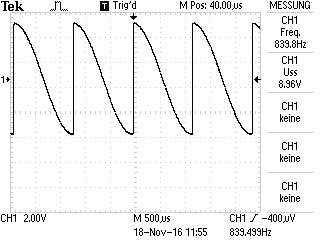
\includegraphics[width=\textwidth]{Bilder/15.jpg}
\caption{$\varphi = 15\si{\degree}$}
\label{fig:1}
\end{minipage}
\hspace{10pt}
\vspace{5pt}
\begin{minipage}[t]{0.3\textwidth}
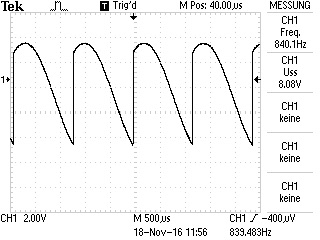
\includegraphics[width=\textwidth]{Bilder/45.jpg}
\caption{$\varphi = 45\si{\degree}$}
\label{fig:2}
\end{minipage}
\hspace{10pt}
\vspace{5pt}
\begin{minipage}[t]{0.3\textwidth}
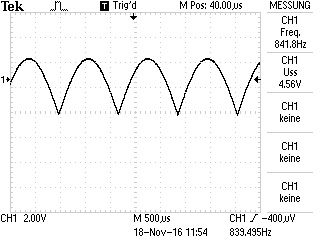
\includegraphics[width=\textwidth]{Bilder/105.jpg}
\caption{$\varphi = 105\si{\degree}$}
\label{fig:3}
\end{minipage}
\hspace{10pt}
\vspace{5pt}
\begin{minipage}[t]{0.3\textwidth}
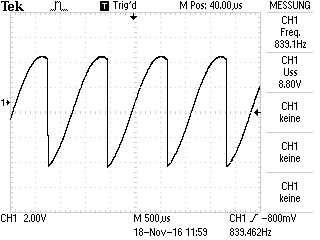
\includegraphics[width=\textwidth]{Bilder/165.jpg}
\caption{$\varphi = 165\si{\degree}$}
\label{fig:4}
\end{minipage}
\hspace{12pt}
\vspace{5pt}
\begin{minipage}[t]{0.3\textwidth}
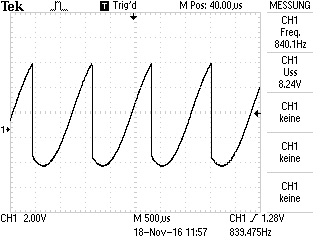
\includegraphics[width=\textwidth]{Bilder/225.jpg}
\caption{$\varphi = 225\si{\degree}$}
\label{fig:5}
\end{minipage}
\hspace{12pt}
\vspace{5pt}
\begin{minipage}[t]{0.3\textwidth}
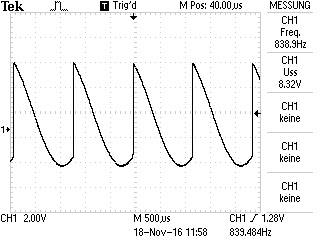
\includegraphics[width=\textwidth]{Bilder/330.jpg}
\caption{$\varphi = 330\si{\degree}$}
\label{fig:6}
\end{minipage}
\hspace{12pt}
\vspace{5pt}
\end{figure}

In den Abbildungen \ref{fig:1} bis \ref{fig:6} sind die Spannungskurven für unterschiedliche Phasen
zu sehen. Hierbei wird weder der Tiefpassfilter noch der Rausch-Generator eingeschaltet. \\
Abbildung \ref{fig:1} zeigt eine sehr steile negative Flanke und spitze Extrema. Abbildung \ref{fig:2}
zeigt auch sehr steile negative Flanken, jedoch sind die Hochpunkte abgerundet. In Abbildung \ref{fig:3}
sieht der Verlauf ungefähr wie der Betrag der Sinus-Kurve aus. In Abbildung \ref{fig:4}
ist die negative Flanke sehr steil, die Hochpunkte sind abgerundet und die Tiefpunkte spitz.
Der Graph in Abbildung \ref{fig:5} hat sehr spitze Hochpunkte und eine sehr steile negative Flanke.
Der Graph in der letzten Abbildung \ref{fig:6} sieht aus wie der Graph aus Abbildung \ref{fig:5}, nur
das er an der y-Achse gespiegelt ist.

\newpage

\begin{figure}[!h]
\begin{minipage}[t]{0.3\textwidth}
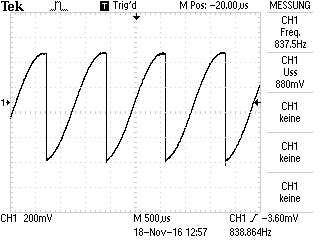
\includegraphics[width=\textwidth]{Bilder/Rausch0.jpg}
\caption{$\varphi = 0\si{\degree}$}
\label{fig:7}
\end{minipage}
\hspace{10pt}
\vspace{5pt}
\begin{minipage}[t]{0.3\textwidth}
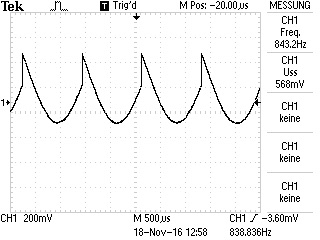
\includegraphics[width=\textwidth]{Bilder/Rausch120.jpg}
\caption{$\varphi = 45\si{\degree}$}
\label{fig:8}
\end{minipage}
\hspace{10pt}
\vspace{5pt}
\begin{minipage}[t]{0.3\textwidth}
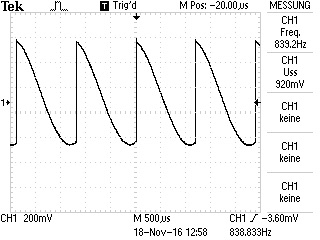
\includegraphics[width=\textwidth]{Bilder/Rausch165.jpg}
\caption{$\varphi = 90\si{\degree}$}
\label{fig:9}
\end{minipage}
\hspace{10pt}
\vspace{5pt}
\begin{minipage}[t]{0.3\textwidth}
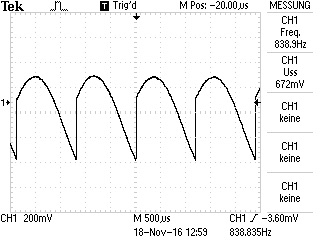
\includegraphics[width=\textwidth]{Bilder/Rausch240.jpg}
\caption{$\varphi = 135\si{\degree}$}
\label{fig:10}
\end{minipage}
\hspace{12pt}
\vspace{5pt}
\begin{minipage}[t]{0.3\textwidth}
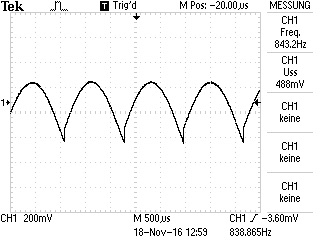
\includegraphics[width=\textwidth]{Bilder/Rausch270.jpg}
\caption{$\varphi = 180\si{\degree}$}
\label{fig:11}
\end{minipage}
\hspace{12pt}
\vspace{5pt}
\begin{minipage}[t]{0.3\textwidth}
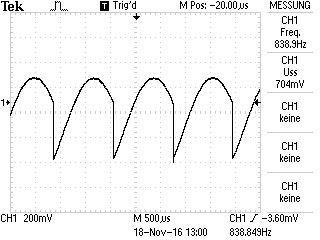
\includegraphics[width=\textwidth]{Bilder/Rausch315.jpg}
\caption{$\varphi = 180\si{\degree}$}
\label{fig:12}
\end{minipage}
\hspace{12pt}
\vspace{5pt}
\end{figure}

In den Abbildungen \ref{fig:7} bis \ref{fig:12} sind die Spannungskurven mit
eingeschaltetem Rausch-Generator zu sehen. Der Tiefpassfilter ist weiterhin ausgeschaltet. \\

\newpage

Im zweiten Teil der Auswertung wird die Abhängigkeit der Ausgangsspannung zur Phasenverschiebung
betrachtet. Hier wird sowohl mit, als auch ohne Rausch-Generator gemessen. Zur besseren
Darstellung wird $\varphi$ gegen $U_\text{out}$ geplottet. Diese Werte sind in Tabelle \ref{tab:b} einzusehen.

\begin{figure}[H]
  \centering
  \includegraphics[width=1.0\textwidth]{Bilder/phi.pdf}
  \caption{U$_\text{out}$ in Abhängigkeit von $\varphi$.}
  \label{fig:Uout}
\end{figure}

Die Funktionen in Grafik \ref{fig:Uout} lassen einen cosinusförmigen Verlauf erkennen. \\

\newpage


Im letzten Teil der Auswertung wird untersucht, bei welcher maximalen Entfernung $r$
eine Photodiode keinen Lichtimpuls einer LED mehr aufnimmt. Dabei wird die eingehende Spannung $U$
gegen den Abstand $r$ mit den Messdaten aus Tabelle \ref{tab:licht} geplottet.
Zu Beginn wird eine Dunkelmessung durchgeführt, welche einen Wert von $U = 0.06 \,\mV$
ergibt. Dieser Wert wird bei den aufgenommenen Spannungswerten im Folgenden direkt
abgezogen.

\begin{table}[H]
  \centering
    \begin{tabular}{cccc}
      \toprule
      {$r \,/ \cm$} & {$U \, / \mV$} & {$r \,/\cm$} & {$U \,/ \mV$} \\
      \midrule
       0  &  2.100   &   22  &  0.125 \\
       2  &  1.200   &   24  &  0.125 \\
       4  &  0.775   &   26  &  0.100 \\
       6  &  0.525   &   28  &  0.100 \\
       8  &  0.375   &   30  &  0.100 \\
      10  &  0.300   &   32  &  0.100 \\
      12  &  0.250   &   34  &  0.075 \\
      14  &  0.200   &   36  &  0.075 \\
      16  &  0.150   &   38  &  0.075 \\
      18  &  0.150   &   40  &  0.075 \\
      20  &  0.125   &  \hrulefill     &  \hrulefill      \\
      \bottomrule
    \end{tabular}
    \caption{Messwerte des Abstands der LED/PD Messung}
    \label{tab:licht}
\end{table}

\begin{figure}[H]
  \centering
  \includegraphics[width=\textwidth]{Bilder/Plot_Photodiode.pdf}
  \caption{U in Abhängigkeit von r}
  \label{fig:led}
\end{figure}

In Grafik \ref{fig:led} ist zu erkennen, dass die Spannung exponentiell zum Abstand
abnimmt. Daraus folgt:

\begin{equation*}
  U \propto \frac{1}{r^2}
\end{equation*}
Der Graph wird mit
\begin{equation}
U = A + \frac{b}{(r+C)^2} \notag
\end{equation}
gefittet.
Dabei ergeben sich die Parameter:
\begin{align*}
  a &= (-0.027 ± 0.005) \; \si{\milli\volt} \\
  b &= (69 ± 2)    \;   \si{\milli\volt\cdot\centi\square\meter}        \\
  c &= (-4.2 ± 0.1) \; \si{\centi\meter}
\end{align*}
\\
Nun wird die Ausgangsspannung gegen $1/r^2$ geplottet, damit ein linearer Fit mit ipython durchgeführt
werden kann.

\begin{figure}[!h]
\centering
\includegraphics[width=\textwidth]{Bilder/photo.pdf}
\caption{Lineare Regression}
\label{fig:lin}
\end{figure}

Die Parameter der Ausgleichgeraden in Grafik \ref{fig:lin} lauten:

\begin{align*}
    a &= (194 ± 9) \; \si{\milli\volt\per\square\centi\meter} \\
    b &= (-0.14 ± 0.03) \; \si{\milli\volt}
\end{align*}

\newpage
\section{Diskussion}
Die Abweichungen der Einzelmesungen für die Fourier-Analyse ergeben sich aus der Formel
\begin{equation}
  \sigma = \frac{a_\su{theo}-a_\su{exp}}{a_\su{theo}}.
\end{equation}
Die jeweiligen Werte wurden dabei schon in der dazugehörigen Tabelle eingetragen.

Für die Abweichung der gesamten Kurve wird Formel \eqref{eqn:fehler} verwendet.
Der Fit der Dreieckspannung weicht somit um $50\,\%$ ab, der Fit der Rechteckspannung
um $19\,\%$ und der Fit der Sägezahnspannung zeigt keine Abweichung.

\noindent Die hohe Abweichung bei der Dreieckspannung ergibt sich daraus, dass wir nur drei Werte genau
einstellen konnten. Bei dem vierten Wert sollte wir $38 \mV$ einstellen, jedoch
ließ sich die Spannung nur bis zu einem Minimalwert von $48 \mV$ einstellen. Diesen
Wert haben wir aber trotzdem noch in die Messung mit einbezogen.

\printbibliography %Zitieren funktioniert noch nicht richtig
\end{document}
